\documentclass[a4paper,twocolumn]{article}

\usepackage[T1]{fontenc}
\usepackage{lmodern}

% Paket za hrvatski jezik neispravno izostavlja toèke iza naslova,
% to ispravljamo zadavanjem novih funkcija za numeriranje koje stavljaju
% toèku.
\makeatletter
\renewcommand\thesection{\@arabic\c@section.}
\renewcommand\thesubsection{\thesection\@arabic\c@subsection.}
\renewcommand\thesubsubsection{\thesubsection\@arabic\c@subsubsection.}
\renewcommand\theequation{\@arabic\c@equation}
\renewcommand\thefigure{\@arabic\c@figure.}
\renewcommand\thetable{\@arabic\c@table.} 
\makeatother

% Ostali korisni paketi.
\RequirePackage{graphicx}
\RequirePackage{hyperref}
\RequirePackage{amssymb}
\RequirePackage{amsmath}
\usepackage{float}

% Ovdje zapoèinje èlanak.
\begin{document}
	
	% Navedite naslov i autore. Datume se automatski postavlja na datum kreiranja dokumenta,
	% no može se promijeniti zadavanjem \date{30. veljaèe, 2004.}
	\title{Paralelna realizacija metoda za obradu slike pomoću NVIDIA CUDA tehnologije} 
	\author{Anabel Dautović, Ita ?, Lana ?, Valeria ?, Marko Haralović, Dino Babić}
	\maketitle
	
	% Svako poglavlje zapoèinje sa \section{Ime poglavlja} ako želimo da bude numerirano,
	% a sa \section*{Ime poglavlja} ako ne želimo da bude numerirano.
	
	\section*{Sažetak}
	Sažetak od stotinjak riječi spominje najvažnije
	teme koje su obrađene u daljnjem tekstu. Tu bi vjerojatno ukratko trebalo napisati o 
	implementacijama koje smo napravili	
	
	
	\section{Uvod}
	Uvod sadrži kratki opis područja, zašto je ono
	važno i koje su primjene. Mislim da bi tu trebalo pisati o području obrade slike, zašto je važno i koje su njegove primjene.
	
	
	\section{Opis područja i aktivnosti u svijetu}
	Opis područja je dataljniji prikaz područja uljučujući
	teoretske osnove i primjene.
	U svakom tehničkom izvještaju ili članku uobičajeno
	je uz svako navođenje rezultata istraživanja i
	primjena razmatranih metoda navesti i poznate istraživačke
	grupe ili laboratoriji u svijetu, odnosno
	referencirati se na objavljene radove, npr. piramidalne
	sheme za brzo bogaćenje pokazale su se iznimno
	uspješne.
	
	Mislim da bi ovdje trebalo pisati o razvoju grafičkih kartica i njihovoj primjeni u produčju obrade slike, koje su razlike i prednosti u odnosu na CPU. Možda malo predstaviti i NVIDIU kao kompaniju, zašto se ona istakla i navesti neke druge prizvođače grafičkih kartica i zašto oni nisu toliko popularni kada je u pitanju primjena grafičkih kartica u računarske svrhe. Također, možda i detaljnije opisati kako uopće rade grafičke kartice.
	
	\section{Pregled implementacija metoda za obradu slika pomoću NVIDIA CUDA tehnologije}
	Ovdje bi za svaku metdou opisao što ona radi, dakle što na primjer radi Canny edge detector i kako to radi, usporedio vremensku razliku između naše implemnentacije na cpu i gpu, ali i ako opencv ima implementaciju tog algoritma onda bih dodao i njega u vremensku usporedbu. Također, treba provjeriti da naša implementacija radi jednako dobro, znači samo provućemo istu sliku kroz našu i opencv implementaciju i prikažemo da su rezultati jednaki ili da se vrlo malo razlikuju. 
	
	
	\subsection{Usporedba maričnog množenja na CPU i GPU te primjena nad transformacijama slike}
	
	Opis metoda slijedi\dots
	
	\subsection{Implementacija metoda za detekciju rubova u slici}
	
	Opis metoda slijedi\dots
	
	\subsection{Implementacija algoritma grupiranje s K srednjih vrijednosti za segmentaciju slike}
	
	Opis metoda slijedi\dots
	
	\subsection{Implementacija neuronske mreže za klasifikaciju rukom pisanih znamenaka}
	
	U ovom poglavlju razmotrit ćemo implementaciju neuronske mreže za klasifikaciju rukom pisanih brojeva. Obje implementacije napisane su u programskom jeziku Python. Verzija koja se izvodu na CPU zasniva se na biblioteci NumPy, dok se verzija koja se izvodi na GPU zasniva na biblioteci CuPy. \newline
	Za treniranje modela korišten je MNIST skup podataka, koji sadrži 60,000 slika rukom pisanih znamenaka. Svaka slika je veličine 28x28 piksela. Prilikom učitavanja skupa podataka, slike su povećane na veličinu 128x128 piksela jer je originalna veličina slika premala da bi se uočile prednosti izvođenja na grafičkim karticama. Naime, treniranje modela s originalnom veličinom slika bilo je sporije na grafičkoj kartici nego na procesoru. Iako se matrične operacije daleko brže izvode na grafičkim karticama, prenošenje podataka na grafičku karticu vremenski je skupo. U slučaju kada imamo malo podataka, vremenski je isplativije izvršiti operacije na procesoru nego prenositi podatke na grafičku karticu i natrag. \newline
	Model u ulaznom sloju ima 16,384 neurona. Skriveni sloj sadrži 30 neurona, dok izlazni sloj ima 10 neurona jer toliko imamo mogućih klasa. Za treniranje modela koristili smo stohastički gradijentni spust, dok smo kao aktivacijsku funkciju koristili sigmoidnu funkciju.
	Oba modela trenirali smo 10 epoha te su im točnosti na testnom skupu podataka bile približno jednake. Treniranje modela koji se izvršavao na procesoru je trajalo 1145 sekundi, dok je treniranje modela koji se izvršavao na grafičkoj kartici trajalo 67 sekundi. Grafička usporedba prikazana je na slici \ref{fig:cnn_training_time_comparison}. \newline
	Vremenska ušteda je značajna. Verzija modela koja se izvršava na grafičkoj kartici također radi brže predikcije, te predikciju za istu sliku izvršava gotovo deset puta brže nego model koji se izvršava na procesoru.
	
	\begin{figure}[H]
		\centering
		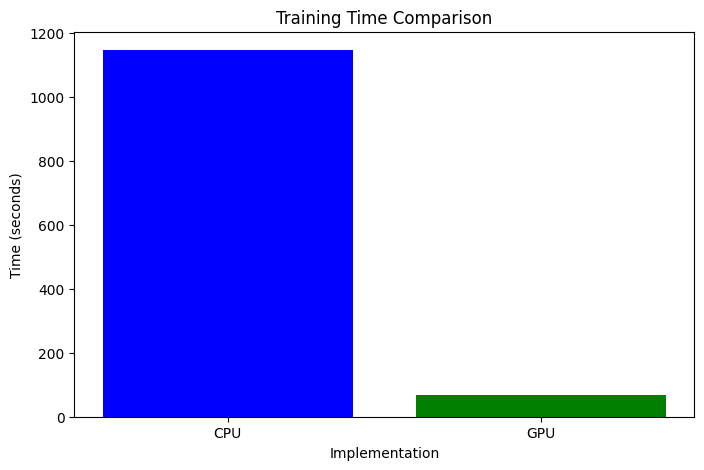
\includegraphics[width=0.9\linewidth]{slike/cnn_training_time_comparison.png} 
		\caption{Prikaz usporedbe vremena treniranja modela koji se izvršavaju na procesoru i na grafičkoj kartici.}
		\label{fig:cnn_training_time_comparison}
	\end{figure} 
	
 	
	
	\subsection{Ostale metode za obradu slike}
	
	Opis metoda slijedi\dots
	
	\section{Zaključak}
	Zaključak treba istaknuti i diskutirati najvažnije rezultate
	iznesene u tekstu i sugerirati eventualne buduće
	trendove.
	
	
	% Literatura se automatski generira iz zadane liste. Svaki od elemenata liste
	% zapoèinje s oznakom, npr. \bibitem{davies}. U tekstu se referenca na èlanak
	% ili knjigu dobiva s \cite{davies}.
	\begin{thebibliography}{25}
		
		\bibitem{davies}
		E.~R.~Davies.
		Machine vision: Theory, Algorithms, Practicalities.
		Academic Press, London, 2. edition, 1997.
		
		\bibitem{wood}
		J.~Lampinen, S.~Smolander, O.~Silv\'{e}n and H. Kauppinen.
		Wood defect recognition: A comparative study,
		Workshop on Machine Vision for Advanced Production, Oulu, Finland, p. 7, 1994.
		
		\bibitem{izopovrsine}
		T.~Itoh i K. Koyyamada.
		Isosurface generation by using extrema graphs,
		Proceedings of Visualization '94, 1994, pp.~77-83, IEEE Computer Society Press, Los Alamitos, CA.
		
		\bibitem{getrichquick}
		J.~User.
		A new efficient algorithm for making money,
		http://www.rich.quick/.
		
	\end{thebibliography} 
	
\end{document} 